\section{Neural Networks and Deep Learning}
\begin{frame}{}
    \LARGE Part 3: \textbf{Neural Networks and Deep Learning}
\end{frame}

\begin{frame}{What is Deep Learning?}
    \centering
    \Large
    Deep Learning is simply \textbf{Machine Learning}...

    \vspace{0.5em}
    ...but powered by \textbf{Artificial Neural Networks} with many layers.

    \vspace{1.5em}
    \normalsize
    \begin{itemize}
        \item \textbf{``Neural'':} Loosely inspired by the brain's neurons.
        \item \textbf{``Deep'':} Refers to the number of layers (depth).
    \end{itemize}

    \vspace{1em}
    \textit{It is the technology behind face unlock, voice assistants, translation and ChatGPT.}
\end{frame}

\begin{frame}{The Artificial Neuron: A Tiny Decision Maker}
    \textit{Should I go out tonight?}

    \vspace{0.3em}
    \centering
    \begin{tikzpicture}[
        inp/.style={rectangle, draw, rounded corners, fill=KAUSTblue!8, text width=3.2cm,
                    align=center, minimum height=0.8cm, font=\small},
        line/.style={draw, -{Latex[length=3mm]}}]
        \node[inp] (a) at (0,1.25) {Is the weather nice?};
        \node[inp] (b) at (0,0) {Are my friends going?};
        \node[inp] (c) at (0,-1.25) {Is it close to home?};
        \node[circle, draw, thick, fill=orange!20, minimum size=2.1cm, align=center, font=\small\bfseries]
            (n) at (6,0) {Weigh\\it all up};
        \node[rectangle, draw, rounded corners, fill=green!12, minimum height=0.9cm, font=\small\bfseries]
            (o) at (10.3,0) {Go / Stay home};
        \path[line, line width=1.2pt] (a.east) -- node[above, sloped, font=\scriptsize] {matters a bit} (n);
        \path[line, line width=3pt] (b.east) -- node[above, font=\scriptsize] {matters a lot} (n);
        \path[line, line width=0.5pt] (c.east) -- node[below, sloped, font=\scriptsize] {barely matters} (n);
        \path[line, thick] (n) -- (o);
    \end{tikzpicture}

    \vspace{0.6em}
    \raggedright
    \begin{itemize}
        \setlength\itemsep{0.3em}
        \item A neuron takes several inputs and gives each one an \textbf{importance}.
        \item It combines them and produces one output.
        \item \textbf{Learning} means finding the right importance for every input.
    \end{itemize}
\end{frame}

\begin{frame}{The Neuron in One Line}
    \begin{block}{}
        \centering
        $z = w_1 x_1 + w_2 x_2 + w_3 x_3 + b$ \qquad then \qquad output $= f(z)$
    \end{block}

    \vspace{0.3em}
    \begin{columns}[T]
        \begin{column}{0.47\textwidth}
            \begin{itemize}
                \setlength\itemsep{0.4em}
                \item $x$: the \textbf{inputs} (1 = yes, 0 = no)
                \item $w$: the \textbf{weights} --- how much each input matters
                \item $b$: the \textbf{bias} --- how easy the neuron is to convince
                \item $f$: the \textbf{activation} --- here: say ``go'' if $z > 0$
            \end{itemize}
        \end{column}
        \begin{column}{0.5\textwidth}
            \begin{tcolorbox}[colback=blue!5, colframe=blue!50, title=\textbf{Worked example}]
                \small
                Nice weather: $x_1 = 1$, \; $w_1 = 2$\\
                Friends going: $x_2 = 1$, \; $w_2 = 5$\\
                Close to home: $x_3 = 0$, \; $w_3 = 0.5$\\
                Bias: $b = -4$

                \vspace{0.4em}
                $z = 2(1) + 5(1) + 0.5(0) - 4 = 3$

                \vspace{0.2em}
                $z > 0 \;\Rightarrow\;$ \textbf{Go!}
            \end{tcolorbox}
        \end{column}
    \end{columns}
\end{frame}

\begin{frame}{From One Neuron to a Network}
    \begin{columns}[c]
        \begin{column}{0.55\textwidth}
            \centering
            \begin{tikzpicture}[scale=0.85,
                neuron/.style={circle, draw, thick, minimum size=0.55cm, inner sep=0pt}]
                \foreach \i in {1,2,3}
                    \node[neuron, fill=KAUSTblue!20] (I\i) at (0,2.25-\i*1.5+0.75) {};
                \foreach \i in {1,2,3,4}
                    \node[neuron, fill=orange!25] (H\i) at (2.4,3-\i*1.2) {};
                \foreach \i in {1,2,3,4}
                    \node[neuron, fill=orange!25] (G\i) at (4.8,3-\i*1.2) {};
                \foreach \i in {1,2}
                    \node[neuron, fill=green!25] (O\i) at (7.2,1.8-\i*1.2) {};
                \foreach \i in {1,2,3} \foreach \j in {1,2,3,4} \draw[gray] (I\i) -- (H\j);
                \foreach \i in {1,2,3,4} \foreach \j in {1,2,3,4} \draw[gray] (H\i) -- (G\j);
                \foreach \i in {1,2,3,4} \foreach \j in {1,2} \draw[gray] (G\i) -- (O\j);
                \node[font=\scriptsize, align=center] at (0,-2.4) {Input\\layer};
                \node[font=\scriptsize, align=center] at (3.6,-2.4) {Hidden layers};
                \node[font=\scriptsize, align=center] at (7.2,-2.4) {Output\\layer};
            \end{tikzpicture}
        \end{column}
        \begin{column}{0.43\textwidth}
            \begin{itemize}
                \setlength\itemsep{0.7em}
                \item One neuron can only make a very simple decision.
                \item Connect many of them in \textbf{layers}, and each layer builds on the one before.
                \item Every line is a connection with its own importance.
                \item Modern networks have \textbf{billions} of these connections.
            \end{itemize}
        \end{column}
    \end{columns}
\end{frame}

\begin{frame}{What Do the Layers Learn?}
    \centering
    \includegraphics[width=0.8\linewidth,height=0.6\textheight,keepaspectratio]{images/nn_exampe_google_guy.png}

    \vspace{0.6em}
    \small
    \begin{tabular}{@{}>{\centering\arraybackslash}p{0.2\linewidth}
                       >{\centering\arraybackslash}p{0.2\linewidth}
                       >{\centering\arraybackslash}p{0.2\linewidth}@{}}
        \textbf{Early layers} & \textbf{Middle layers} & \textbf{Later layers} \\
        edges and lines & eyes, noses, mouths & whole faces \\
    \end{tabular}
    \normalsize

    \vspace{0.5em}
    \textit{Nobody tells the network to look for eyes. It works this out from the examples.}
\end{frame}

\begin{frame}{How Does a Network Learn?}
    \centering
    \begin{tikzpicture}[
        stepbox/.style={rectangle, draw, rounded corners, thick, minimum height=1.1cm,
                     text width=2.6cm, align=center, font=\small\bfseries},
        line/.style={draw, -{Latex[length=3mm]}, thick}]
        \node[stepbox, fill=KAUSTblue!10] (guess) at (0,0) {1. Make a guess};
        \node[stepbox, fill=KAred!10] (check) at (4.4,0) {2. Measure the loss};
        \node[stepbox, fill=orange!15] (adjust) at (8.8,0) {3. Adjust the weights a little};
        \path[line] (guess) -- (check);
        \path[line] (check) -- (adjust);
        \path[line] (adjust.south) -- ++(0,-0.7) -| node[pos=0.25, below, font=\small] {repeat millions of times} (guess.south);
    \end{tikzpicture}

    \vspace{0.8em}
    \raggedright
    \begin{itemize}
        \setlength\itemsep{0.4em}
        \item At the start the network knows nothing --- its guesses are random.
        \item Each mistake nudges the weights so the next guess is slightly better.
        \item It is like practising free throws: shoot, see where the ball went, correct, repeat.
    \end{itemize}
\end{frame}

\begin{frame}{Gradient Descent: Walking Downhill}
    \begin{columns}[c]
        \begin{column}{0.5\textwidth}
            \centering
            \begin{tikzpicture}[scale=0.95]
                \draw[->, thick] (0,0) -- (6.2,0) node[below left] {\scriptsize value of one weight};
                \draw[->, thick] (0,0) -- (0,4.2) node[above] {\scriptsize loss};
                \draw[KAUSTblue, very thick, domain=0.6:5.6, samples=50]
                    plot (\x, {0.55*(\x-3.4)*(\x-3.4)+0.5});
                \foreach \x in {0.9,1.7,2.4,2.9}
                    \filldraw[KAred] (\x, {0.55*(\x-3.4)*(\x-3.4)+0.5}) circle (3pt);
                \foreach \a/\b in {0.9/1.7,1.7/2.4,2.4/2.9}
                    \draw[-{Latex[length=2mm]}, KAred, thick]
                        (\a, {0.55*(\a-3.4)*(\a-3.4)+0.75}) -- (\b, {0.55*(\b-3.4)*(\b-3.4)+0.75});
                \node[font=\scriptsize, align=center] at (3.4,0.2) {lowest loss};
            \end{tikzpicture}
        \end{column}
        \begin{column}{0.48\textwidth}
            \begin{itemize}
                \setlength\itemsep{0.6em}
                \item Imagine the loss as a valley. We want to reach the bottom.
                \item At each step, look at the \textbf{slope} and move a little downhill.
            \end{itemize}

            \vspace{0.6em}
            \begin{block}{The update rule}
                \centering
                $w_{\text{new}} = w_{\text{old}} - \text{learning rate} \times \text{slope}$
            \end{block}

            \vspace{0.3em}
            \small The \textbf{learning rate} is the step size: too small is slow, too large overshoots.
        \end{column}
    \end{columns}
\end{frame}

\begin{frame}{Why Now?}
    \textit{Neural networks are not new. The ideas date back decades. But three things changed:}

    \begin{columns}[c]
        \begin{column}{0.4\textwidth}
            \begin{enumerate}
                \setlength\itemsep{0.8em}
                \item More \textbf{data} \\
                {\small (internet, phones, sensors)}
                \item Faster \textbf{computers} \\
                {\small (graphics chips, cloud computing)}
                \item Better \textbf{methods} \\
                {\small (new ways to build and train networks)}
            \end{enumerate}
        \end{column}

        \begin{column}{0.5\textwidth}
            \centering
            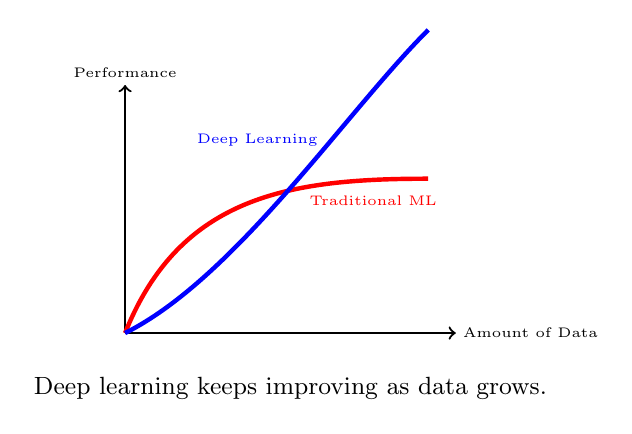
\begin{tikzpicture}[scale=0.7]
            \tiny
                \draw[->, thick] (0,0) -- (6,0) node[right] {Amount of Data};
                \draw[->, thick] (0,0) -- (0,4.5) node[above] {Performance};
                \draw[red, ultra thick] (0,0) .. controls (1,2.5) and (3,2.8) .. (5.5,2.8);
                \node[red] at (4.5, 2.4) {Traditional ML};
                \draw[blue, ultra thick] (0,0) .. controls (2,1) and (4,4) .. (5.5,5.5);
                \node[blue] at (2.4, 3.5) {Deep Learning};
                \node[align=center, font=\small] at (3, -1) {Deep learning keeps improving as data grows.};
            \end{tikzpicture}
        \end{column}
    \end{columns}
\end{frame}
